\begin{figure}[!h]
  \begin{center}
    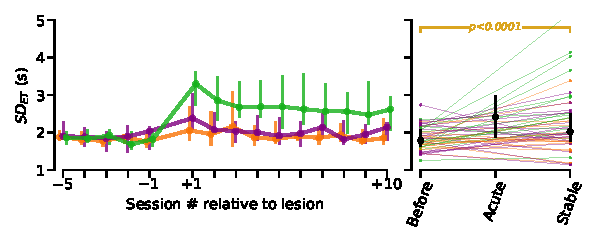
\includegraphics[scale=1]{ch-appendicies/figures/SDofET.pdf}
    \caption[Temporal Variability After Lesion]
    {\textbf{Temporal variability increased after striatal lesions.}
    \textit{Left}: session-by-session standard deviation of entrance times relative to the lesion.
    colored traces show lesion groups (DLS, DMS, DS, same as in \autoref{fig:lesion:task}).
    \textit{Right}: statistical comparison of ET variability.
    Each line represents one animal.
    }
    \label{fig:appendix:SdofET}
  \end{center}
\end{figure}